\documentclass[]{article}
\usepackage{lmodern}
\usepackage{amssymb,amsmath}
\usepackage{ifxetex,ifluatex}
\usepackage{fixltx2e} % provides \textsubscript
\ifnum 0\ifxetex 1\fi\ifluatex 1\fi=0 % if pdftex
  \usepackage[T1]{fontenc}
  \usepackage[utf8]{inputenc}
\else % if luatex or xelatex
  \ifxetex
    \usepackage{mathspec}
  \else
    \usepackage{fontspec}
  \fi
  \defaultfontfeatures{Ligatures=TeX,Scale=MatchLowercase}
\fi
% use upquote if available, for straight quotes in verbatim environments
\IfFileExists{upquote.sty}{\usepackage{upquote}}{}
% use microtype if available
\IfFileExists{microtype.sty}{%
\usepackage{microtype}
\UseMicrotypeSet[protrusion]{basicmath} % disable protrusion for tt fonts
}{}
\usepackage[margin=1in]{geometry}
\usepackage{hyperref}
\hypersetup{unicode=true,
            pdftitle={Individual Analysis},
            pdfauthor={Dario Trujano Ochoa},
            pdfborder={0 0 0},
            breaklinks=true}
\urlstyle{same}  % don't use monospace font for urls
\usepackage{color}
\usepackage{fancyvrb}
\newcommand{\VerbBar}{|}
\newcommand{\VERB}{\Verb[commandchars=\\\{\}]}
\DefineVerbatimEnvironment{Highlighting}{Verbatim}{commandchars=\\\{\}}
% Add ',fontsize=\small' for more characters per line
\usepackage{framed}
\definecolor{shadecolor}{RGB}{248,248,248}
\newenvironment{Shaded}{\begin{snugshade}}{\end{snugshade}}
\newcommand{\KeywordTok}[1]{\textcolor[rgb]{0.13,0.29,0.53}{\textbf{#1}}}
\newcommand{\DataTypeTok}[1]{\textcolor[rgb]{0.13,0.29,0.53}{#1}}
\newcommand{\DecValTok}[1]{\textcolor[rgb]{0.00,0.00,0.81}{#1}}
\newcommand{\BaseNTok}[1]{\textcolor[rgb]{0.00,0.00,0.81}{#1}}
\newcommand{\FloatTok}[1]{\textcolor[rgb]{0.00,0.00,0.81}{#1}}
\newcommand{\ConstantTok}[1]{\textcolor[rgb]{0.00,0.00,0.00}{#1}}
\newcommand{\CharTok}[1]{\textcolor[rgb]{0.31,0.60,0.02}{#1}}
\newcommand{\SpecialCharTok}[1]{\textcolor[rgb]{0.00,0.00,0.00}{#1}}
\newcommand{\StringTok}[1]{\textcolor[rgb]{0.31,0.60,0.02}{#1}}
\newcommand{\VerbatimStringTok}[1]{\textcolor[rgb]{0.31,0.60,0.02}{#1}}
\newcommand{\SpecialStringTok}[1]{\textcolor[rgb]{0.31,0.60,0.02}{#1}}
\newcommand{\ImportTok}[1]{#1}
\newcommand{\CommentTok}[1]{\textcolor[rgb]{0.56,0.35,0.01}{\textit{#1}}}
\newcommand{\DocumentationTok}[1]{\textcolor[rgb]{0.56,0.35,0.01}{\textbf{\textit{#1}}}}
\newcommand{\AnnotationTok}[1]{\textcolor[rgb]{0.56,0.35,0.01}{\textbf{\textit{#1}}}}
\newcommand{\CommentVarTok}[1]{\textcolor[rgb]{0.56,0.35,0.01}{\textbf{\textit{#1}}}}
\newcommand{\OtherTok}[1]{\textcolor[rgb]{0.56,0.35,0.01}{#1}}
\newcommand{\FunctionTok}[1]{\textcolor[rgb]{0.00,0.00,0.00}{#1}}
\newcommand{\VariableTok}[1]{\textcolor[rgb]{0.00,0.00,0.00}{#1}}
\newcommand{\ControlFlowTok}[1]{\textcolor[rgb]{0.13,0.29,0.53}{\textbf{#1}}}
\newcommand{\OperatorTok}[1]{\textcolor[rgb]{0.81,0.36,0.00}{\textbf{#1}}}
\newcommand{\BuiltInTok}[1]{#1}
\newcommand{\ExtensionTok}[1]{#1}
\newcommand{\PreprocessorTok}[1]{\textcolor[rgb]{0.56,0.35,0.01}{\textit{#1}}}
\newcommand{\AttributeTok}[1]{\textcolor[rgb]{0.77,0.63,0.00}{#1}}
\newcommand{\RegionMarkerTok}[1]{#1}
\newcommand{\InformationTok}[1]{\textcolor[rgb]{0.56,0.35,0.01}{\textbf{\textit{#1}}}}
\newcommand{\WarningTok}[1]{\textcolor[rgb]{0.56,0.35,0.01}{\textbf{\textit{#1}}}}
\newcommand{\AlertTok}[1]{\textcolor[rgb]{0.94,0.16,0.16}{#1}}
\newcommand{\ErrorTok}[1]{\textcolor[rgb]{0.64,0.00,0.00}{\textbf{#1}}}
\newcommand{\NormalTok}[1]{#1}
\usepackage{graphicx,grffile}
\makeatletter
\def\maxwidth{\ifdim\Gin@nat@width>\linewidth\linewidth\else\Gin@nat@width\fi}
\def\maxheight{\ifdim\Gin@nat@height>\textheight\textheight\else\Gin@nat@height\fi}
\makeatother
% Scale images if necessary, so that they will not overflow the page
% margins by default, and it is still possible to overwrite the defaults
% using explicit options in \includegraphics[width, height, ...]{}
\setkeys{Gin}{width=\maxwidth,height=\maxheight,keepaspectratio}
\IfFileExists{parskip.sty}{%
\usepackage{parskip}
}{% else
\setlength{\parindent}{0pt}
\setlength{\parskip}{6pt plus 2pt minus 1pt}
}
\setlength{\emergencystretch}{3em}  % prevent overfull lines
\providecommand{\tightlist}{%
  \setlength{\itemsep}{0pt}\setlength{\parskip}{0pt}}
\setcounter{secnumdepth}{0}
% Redefines (sub)paragraphs to behave more like sections
\ifx\paragraph\undefined\else
\let\oldparagraph\paragraph
\renewcommand{\paragraph}[1]{\oldparagraph{#1}\mbox{}}
\fi
\ifx\subparagraph\undefined\else
\let\oldsubparagraph\subparagraph
\renewcommand{\subparagraph}[1]{\oldsubparagraph{#1}\mbox{}}
\fi

%%% Use protect on footnotes to avoid problems with footnotes in titles
\let\rmarkdownfootnote\footnote%
\def\footnote{\protect\rmarkdownfootnote}

%%% Change title format to be more compact
\usepackage{titling}

% Create subtitle command for use in maketitle
\newcommand{\subtitle}[1]{
  \posttitle{
    \begin{center}\large#1\end{center}
    }
}

\setlength{\droptitle}{-2em}
  \title{Individual Analysis}
  \pretitle{\vspace{\droptitle}\centering\huge}
  \posttitle{\par}
  \author{Dario Trujano Ochoa}
  \preauthor{\centering\large\emph}
  \postauthor{\par}
  \date{}
  \predate{}\postdate{}


\begin{document}
\maketitle

{
\setcounter{tocdepth}{2}
\tableofcontents
}
\section{Data}\label{data}

Let's import some data bases previusly created from the treatments:

\begin{Shaded}
\begin{Highlighting}[]
\KeywordTok{getwd}\NormalTok{()}
\end{Highlighting}
\end{Shaded}

\begin{verbatim}
## [1] "D:/Dario/Dropbox/Citizen-Candidate/ArticleCitizenCandidate"
\end{verbatim}

\begin{Shaded}
\begin{Highlighting}[]
\NormalTok{participants_}\DecValTok{305075}\NormalTok{ <-}\StringTok{ }\KeywordTok{read.csv}\NormalTok{(}\StringTok{"data/participants_305075.csv"}\NormalTok{)[,}\DecValTok{2}\OperatorTok{:}\DecValTok{8}\NormalTok{]}
\KeywordTok{colnames}\NormalTok{(participants_}\DecValTok{305075}\NormalTok{)[}\DecValTok{3}\OperatorTok{:}\DecValTok{5}\NormalTok{] <-}\StringTok{ }\KeywordTok{c}\NormalTok{(}\StringTok{"Left"}\NormalTok{, }\StringTok{"Center"}\NormalTok{, }\StringTok{"Right"}\NormalTok{)}
\NormalTok{participants_}\DecValTok{203080}\NormalTok{ <-}\StringTok{ }\KeywordTok{read.csv}\NormalTok{(}\StringTok{"data/participants_203080.csv"}\NormalTok{)[,}\DecValTok{2}\OperatorTok{:}\DecValTok{8}\NormalTok{]}
\KeywordTok{colnames}\NormalTok{(participants_}\DecValTok{203080}\NormalTok{)[}\DecValTok{3}\OperatorTok{:}\DecValTok{5}\NormalTok{] <-}\StringTok{ }\KeywordTok{c}\NormalTok{(}\StringTok{"Left"}\NormalTok{, }\StringTok{"Center"}\NormalTok{, }\StringTok{"Right"}\NormalTok{)}
\end{Highlighting}
\end{Shaded}

and now I merge them

\begin{Shaded}
\begin{Highlighting}[]
\NormalTok{participants <-}\StringTok{ }\KeywordTok{rbind}\NormalTok{(participants_}\DecValTok{305075}\NormalTok{,participants_}\DecValTok{203080}\NormalTok{)}

\NormalTok{treatments <-}\StringTok{ }\KeywordTok{names}\NormalTok{(}\KeywordTok{table}\NormalTok{(participants}\OperatorTok{$}\NormalTok{Game))}
\NormalTok{treatments_names <-}\StringTok{ }\KeywordTok{cbind.data.frame}\NormalTok{(treatments,}
                          \DataTypeTok{NewNames =} \KeywordTok{c}\NormalTok{(}\StringTok{"PLCS"}\NormalTok{,}\StringTok{"PLCA"}\NormalTok{,}\StringTok{"PL"}\NormalTok{,}\StringTok{"PH"}\NormalTok{,}\StringTok{"RL"}\NormalTok{,}\StringTok{"RH"}\NormalTok{))}
\end{Highlighting}
\end{Shaded}

\section{Graphs on Individual
Behavior}\label{graphs-on-individual-behavior}

With the next graphs, we visually analize hetereogeneity among
participants. The entry porportion by individual and by relative
position are displayed; each red line relate data from each participant.
For simplicity, we analize the bahavior according with the relative
position, i.e., 1 stand for the left extreme candidate, 2 for that one
in the middle, and the extreme right candidate is represented by 3. The
precise postiion depends of the treatment.

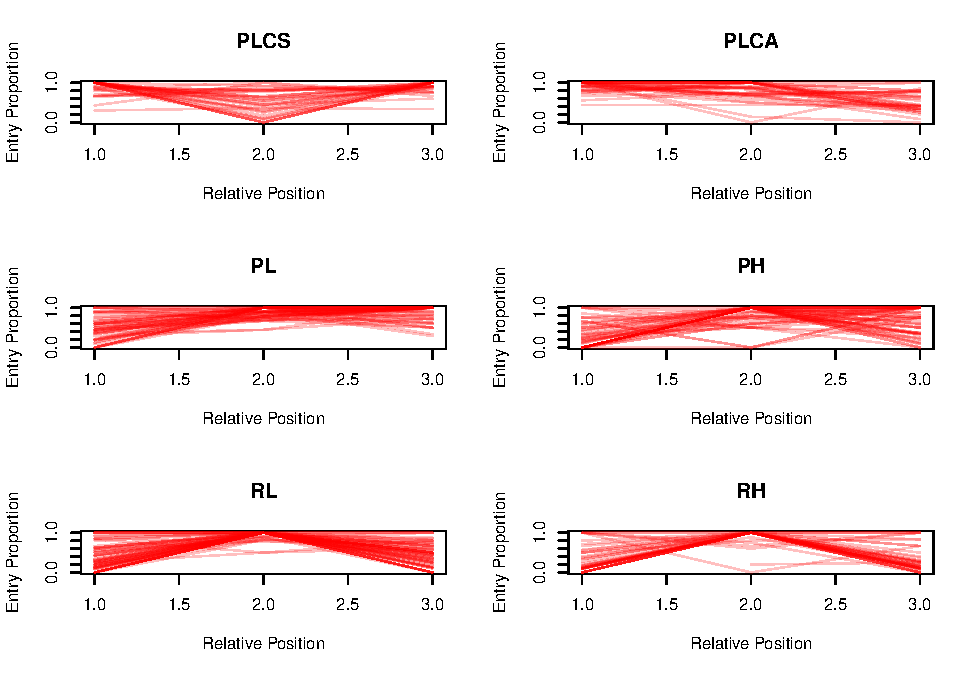
\includegraphics{individual_analysis_report_files/figure-latex/unnamed-chunk-3-1.pdf}

The behavior displayed is very simmilar among participants within
treatments. Some participants deviate from the general path, but they
are rare. Also, we can see that the variance increases for the position
that should not enter according with Nash prediction.

\section{Entry bias}\label{entry-bias}

We considered the hypothesis of a biased decision towards entry.

First, let us consider the parameters of the treatments:

\begin{Shaded}
\begin{Highlighting}[]
\NormalTok{alpha =}\StringTok{ }\FloatTok{0.1} 
\NormalTok{costs =}\StringTok{ }\KeywordTok{c}\NormalTok{(}\DecValTok{5}\NormalTok{,}\DecValTok{5}\NormalTok{,}\DecValTok{5}\NormalTok{,}\DecValTok{20}\NormalTok{,}\DecValTok{5}\NormalTok{,}\DecValTok{20}\NormalTok{) }\CommentTok{#costs in treatments}
\NormalTok{benefit =}\StringTok{ }\DecValTok{25}
\NormalTok{D =}\StringTok{ }\DecValTok{40} \CommentTok{# penalty if no one enters}
\CommentTok{# what everybody does}
\NormalTok{n =}\StringTok{ }\DecValTok{3}         \CommentTok{# numer of players}
\NormalTok{Q_games =}\StringTok{ }\KeywordTok{cbind}\NormalTok{(}\KeywordTok{matrix}\NormalTok{(}\KeywordTok{c}\NormalTok{(}\KeywordTok{c}\NormalTok{(}\DecValTok{30}\NormalTok{, }\DecValTok{50}\NormalTok{, }\DecValTok{70}\NormalTok{),}\KeywordTok{c}\NormalTok{(}\DecValTok{30}\NormalTok{, }\DecValTok{50}\NormalTok{, }\DecValTok{80}\NormalTok{),}\KeywordTok{rep}\NormalTok{(}\KeywordTok{c}\NormalTok{(}\DecValTok{20}\NormalTok{, }\DecValTok{30}\NormalTok{, }\DecValTok{80}\NormalTok{),}\DecValTok{4}\NormalTok{)),}\DataTypeTok{ncol=}\DecValTok{3}\NormalTok{,}\DataTypeTok{nrow=}\DecValTok{6}\NormalTok{,}\DataTypeTok{byrow =}\NormalTok{ T))  }\CommentTok{# ideal points used in the experiment}
\NormalTok{parameters_games <-}\KeywordTok{cbind}\NormalTok{(alpha, costs, benefit,D)}
\KeywordTok{row.names}\NormalTok{(parameters_games) <-}\StringTok{ }\NormalTok{treatments}
\NormalTok{VotingRule <-}\StringTok{ }\KeywordTok{c}\NormalTok{(}\StringTok{"Plurality Rule"}\NormalTok{,}\StringTok{"Plurality Rule"}\NormalTok{,}\StringTok{"Plurality Rule"}\NormalTok{,}\StringTok{"Plurality Rule"}\NormalTok{,}\StringTok{"Run-Off"}\NormalTok{,}\StringTok{"Run-Off"}\NormalTok{)}
\NormalTok{parameters_games2 <-}\StringTok{ }\KeywordTok{data.frame}\NormalTok{(VotingRule,parameters_games,Q_games)}
\NormalTok{game_names <-}\StringTok{  }\NormalTok{treatments_names}\OperatorTok{$}\NormalTok{NewNames}
\KeywordTok{row.names}\NormalTok{(parameters_games2) <-}\StringTok{ }\NormalTok{game_names}
\KeywordTok{colnames}\NormalTok{(parameters_games2)[}\DecValTok{6}\OperatorTok{:}\DecValTok{8}\NormalTok{] <-}\StringTok{ }\KeywordTok{c}\NormalTok{(}\StringTok{"Left"}\NormalTok{, }\StringTok{"Center"}\NormalTok{, }\StringTok{"Right"}\NormalTok{)}
\NormalTok{Equilibria <-}\StringTok{ }\KeywordTok{data.frame}\NormalTok{(}
  \DataTypeTok{Games=}\NormalTok{ game_names,}
  \DataTypeTok{OneCandidate=} \KeywordTok{c}\NormalTok{(}\DecValTok{50}\NormalTok{,}\DecValTok{50}\NormalTok{,}\DecValTok{30}\NormalTok{,}\DecValTok{30}\NormalTok{,}\DecValTok{30}\NormalTok{,}\DecValTok{30}\NormalTok{),}
  \DataTypeTok{TwoCandidate=} \KeywordTok{c}\NormalTok{(}\StringTok{"30, 70"}\NormalTok{,}\OtherTok{NA}\NormalTok{, }\StringTok{"20, 80"}\NormalTok{,}\OtherTok{NA}\NormalTok{,}\OtherTok{NA}\NormalTok{,}\OtherTok{NA}\NormalTok{) )}
\end{Highlighting}
\end{Shaded}

Second, we get the proportion of entry by session.

Finally, we merge the proportion of entry, the proportion of entry by
session, and the expected payoffs of entry by session in a single data
base.

\begin{Shaded}
\begin{Highlighting}[]
\KeywordTok{str}\NormalTok{(entry_proportions_by_session)}
\end{Highlighting}
\end{Shaded}

\begin{verbatim}
##  num [1:16, 1:3] 0.856 0.933 0.881 0.934 0.592 ...
##  - attr(*, "dimnames")=List of 2
##   ..$ : NULL
##   ..$ : chr [1:3] "Left" "Center" "Right"
\end{verbatim}

\begin{Shaded}
\begin{Highlighting}[]
\KeywordTok{write.csv}\NormalTok{(entry_proportions_by_session, }\StringTok{"data/entry_proportions_by_session.csv"}\NormalTok{)}

\NormalTok{participants <-}\StringTok{ }\KeywordTok{cbind.data.frame}\NormalTok{(participants,exp_val_participants,optimal_participants) }
\NormalTok{positions_should_entry <-}\StringTok{ }\KeywordTok{c}\NormalTok{(}\StringTok{"ShouldLeftEntry"}\NormalTok{, }\StringTok{"ShouldCenterEntry"}\NormalTok{,}\StringTok{"ShouldRightEntry"}\NormalTok{)}
\NormalTok{positions_prop_entry <-}\StringTok{ }\KeywordTok{names}\NormalTok{(participants[}\DecValTok{3}\OperatorTok{:}\DecValTok{5}\NormalTok{])}

\NormalTok{errors <-}\StringTok{  }\NormalTok{participants[positions_prop_entry]}\OperatorTok{-}
\StringTok{  }\NormalTok{participants[positions_should_entry] }\CommentTok{# there are 3 participants that no played some position}
\KeywordTok{names}\NormalTok{(errors) <-}\StringTok{ }\KeywordTok{paste}\NormalTok{(}\StringTok{"Errors"}\NormalTok{,}\KeywordTok{names}\NormalTok{(errors))}

\NormalTok{errors1 <-}\StringTok{ }\NormalTok{errors }\OperatorTok{>}\StringTok{ }\DecValTok{0} \CommentTok{# they entry when should not}
\NormalTok{errors2 <-}\StringTok{ }\NormalTok{errors }\OperatorTok{<}\StringTok{ }\DecValTok{0} \CommentTok{# they do not enter when they should }

\NormalTok{Error1 <-}\StringTok{ }\KeywordTok{rowSums}\NormalTok{(errors}\OperatorTok{*}\NormalTok{errors1,}\DataTypeTok{na.rm =}\NormalTok{ T) }\CommentTok{# when players never played some position there is NA}
\NormalTok{Error2 <-}\StringTok{ }\KeywordTok{rowSums}\NormalTok{(errors}\OperatorTok{*}\NormalTok{errors2,}\DataTypeTok{na.rm =}\NormalTok{ T)}

\NormalTok{participants <-}\StringTok{ }\KeywordTok{cbind}\NormalTok{(participants,errors,Error1,Error2)}
\KeywordTok{str}\NormalTok{(participants)}
\end{Highlighting}
\end{Shaded}

\begin{verbatim}
## 'data.frame':    301 obs. of  21 variables:
##  $ Game             : Factor w/ 6 levels "ex70","ex80",..: 1 1 1 1 1 1 1 1 1 1 ...
##  $ Session          : int  1 1 1 1 1 1 1 1 1 1 ...
##  $ Left             : num  0.8 0.9 0.875 0.7 0.636 ...
##  $ Center           : num  0.8 0.8 0.0909 0.7692 0.8571 ...
##  $ Right            : num  0.9 1 1 1 0.917 ...
##  $ Effective_Trials : int  30 30 30 30 30 30 30 30 30 30 ...
##  $ Bankrupcy        : int  0 0 0 0 0 0 1 0 0 0 ...
##  $ LeftEntry        : num  5.46 5.46 5.46 5.46 5.46 ...
##  $ CenterEntry      : num  0.0182 0.0182 0.0182 0.0182 0.0182 ...
##  $ RightEntry       : num  5.45 5.45 5.45 5.45 5.45 ...
##  $ LeftPass         : num  -5.11 -5.11 -5.11 -5.11 -5.11 ...
##  $ CenterPass       : num  -2.74 -2.74 -2.74 -2.74 -2.74 ...
##  $ RightPass        : num  -5.24 -5.24 -5.24 -5.24 -5.24 ...
##  $ ShouldLeftEntry  : logi  TRUE TRUE TRUE TRUE TRUE TRUE ...
##  $ ShouldCenterEntry: logi  TRUE TRUE TRUE TRUE TRUE TRUE ...
##  $ ShouldRightEntry : logi  TRUE TRUE TRUE TRUE TRUE TRUE ...
##  $ Errors Left      : num  -0.2 -0.1 -0.125 -0.3 -0.364 ...
##  $ Errors Center    : num  -0.2 -0.2 -0.909 -0.231 -0.143 ...
##  $ Errors Right     : num  -0.1 0 0 0 -0.0833 ...
##  $ Error1           : num  0 0 0 0 0 0 0 0 0 0 ...
##  $ Error2           : num  -0.5 -0.3 -1.034 -0.531 -0.59 ...
\end{verbatim}

\begin{Shaded}
\begin{Highlighting}[]
\KeywordTok{write.csv}\NormalTok{(participants,}\DataTypeTok{file =} \StringTok{"data/participants.csv"}\NormalTok{)}
\end{Highlighting}
\end{Shaded}

\section{Biased towards entry}\label{biased-towards-entry}

In order to anaize the errror bias, we considered the difference between
the entry proportion and the optimal decision, e.g.~if the optimal
decision was to enter, and the proportion observed was \(0.5\), we
calculate a negative error of \(0.5\). Then, a positive error indicates
overentry, and negative subentry relative with the optimal decision. It
can be seen that erros range from -1 to 1, and cero means optimal
behavior.

We ran the analisis by position, as we saw a diference in the idividual
behavior according with this variable. Also, we analized the treatment
effect over error distributons. In each graph, a density was adjusted
and data from the three positions are set for comparison.

\begin{verbatim}
## Warning: Removed 3 rows containing non-finite values (stat_density).
\end{verbatim}

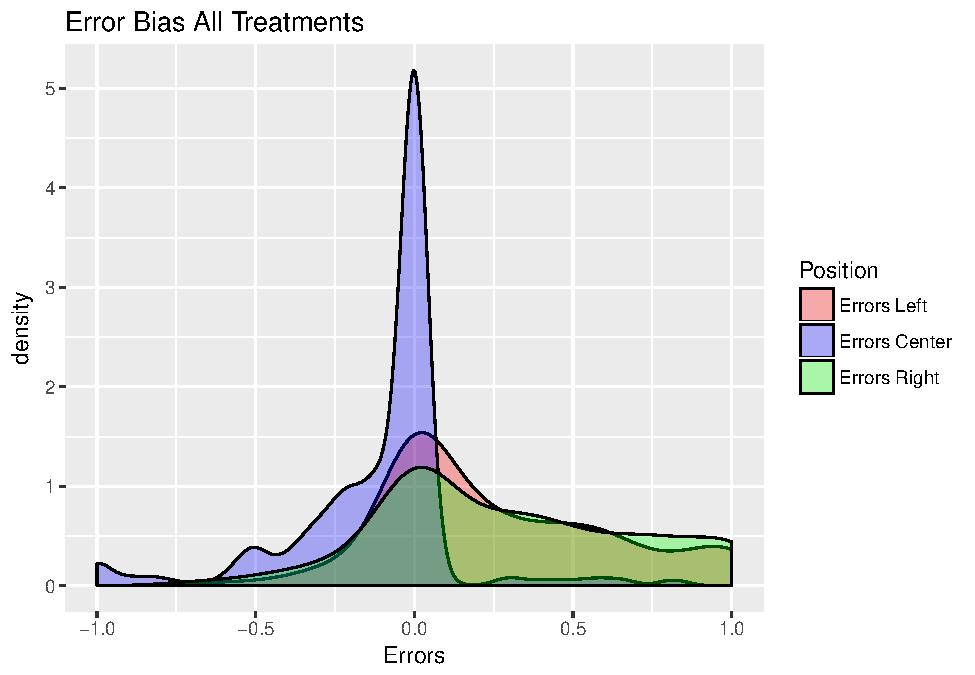
\includegraphics{individual_analysis_report_files/figure-latex/unnamed-chunk-8-1.pdf}

In the graph that shows the joined behavior in all treatments by
position, we can see that extreme positions are more commonly biased
towards over entering, i.e., participants are prone to enter in those
positions even against their interest. On the other hand, in central
position, participants tend to make less mistakes and, if so, they enter
less than predicted.

\subsection{Analysis by Treatment}\label{analysis-by-treatment}

In this section, we analize error distribution in the six treatments.

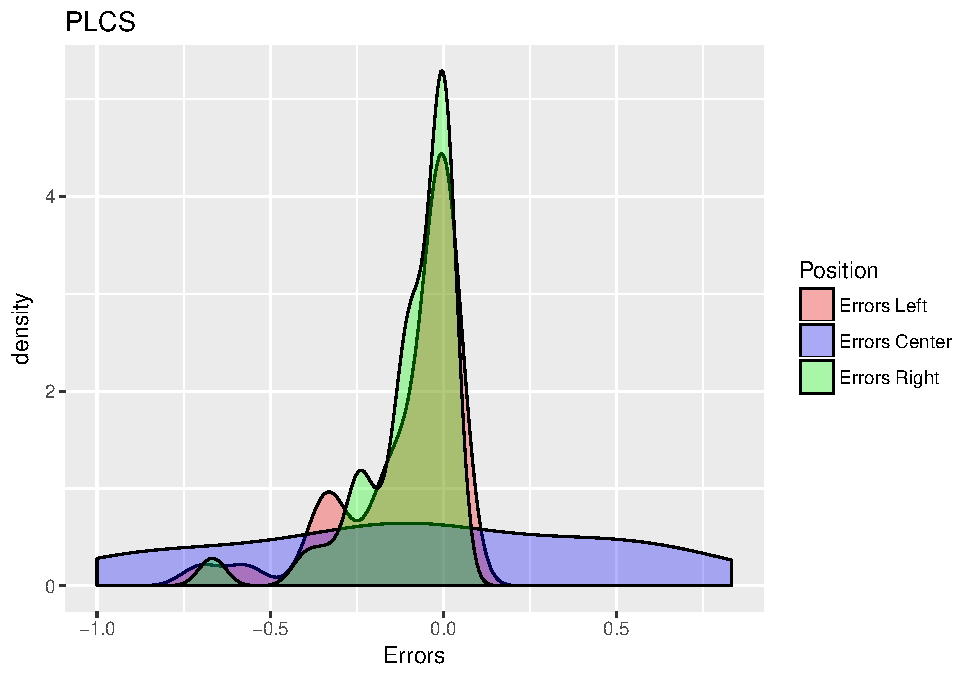
\includegraphics{individual_analysis_report_files/figure-latex/unnamed-chunk-9-1.pdf}
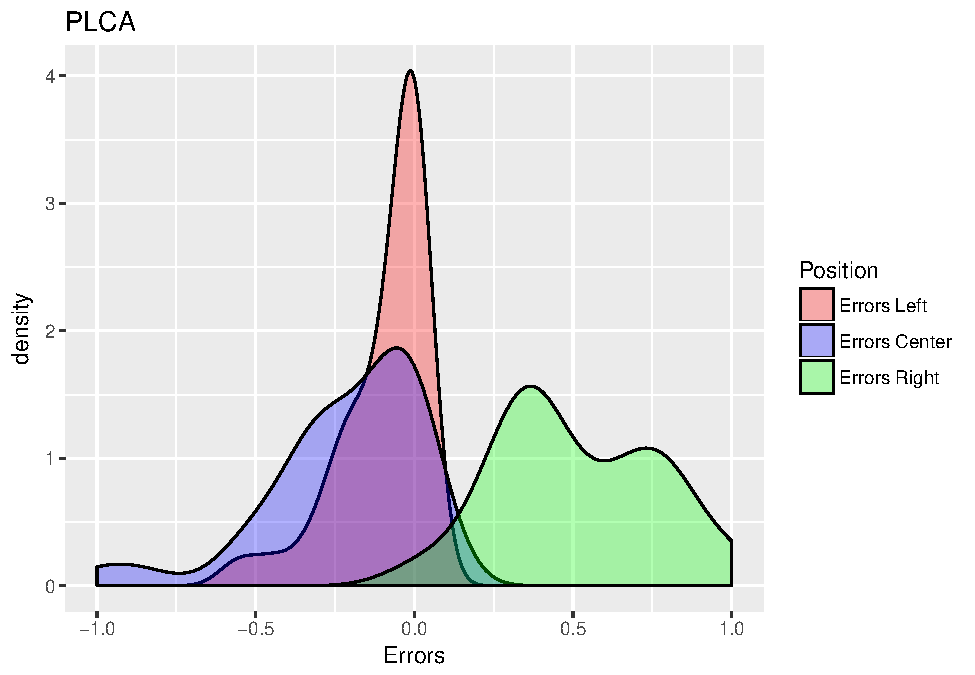
\includegraphics{individual_analysis_report_files/figure-latex/unnamed-chunk-9-2.pdf}

\begin{verbatim}
## Warning: Removed 1 rows containing non-finite values (stat_density).

## Warning: Removed 1 rows containing non-finite values (stat_density).
\end{verbatim}

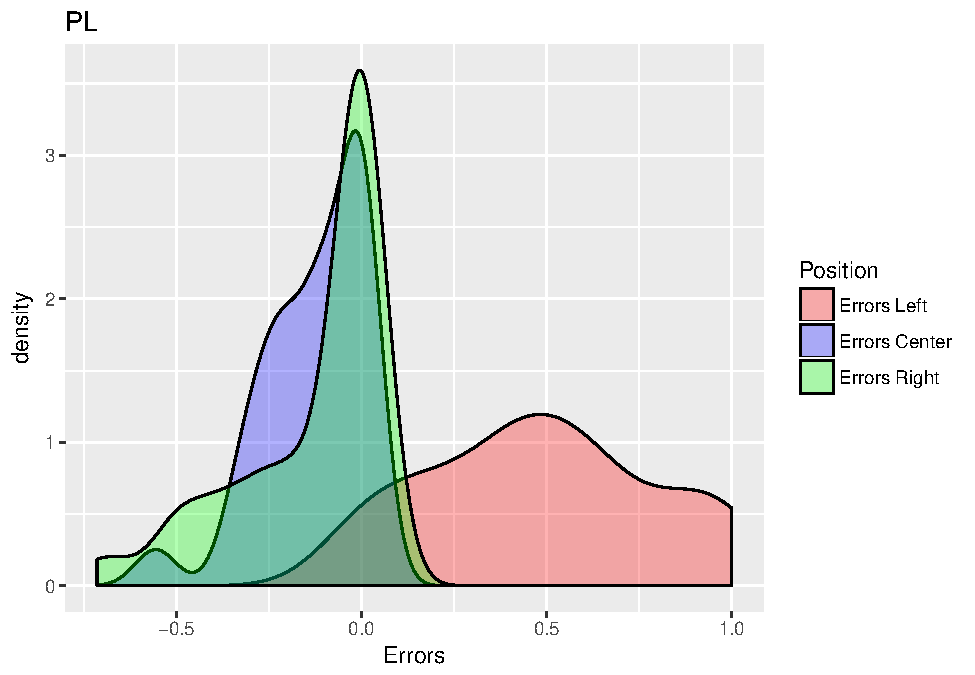
\includegraphics{individual_analysis_report_files/figure-latex/unnamed-chunk-9-3.pdf}

\begin{verbatim}
## Warning: Removed 1 rows containing non-finite values (stat_density).
\end{verbatim}

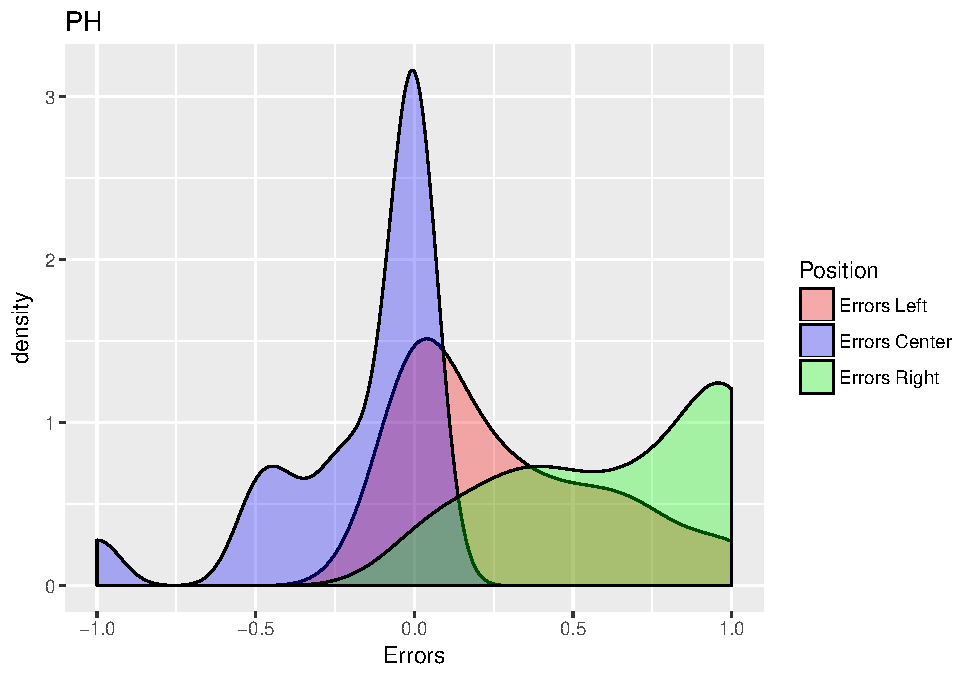
\includegraphics{individual_analysis_report_files/figure-latex/unnamed-chunk-9-4.pdf}

\begin{verbatim}
## Warning: Removed 2 rows containing non-finite values (stat_density).
\end{verbatim}

\begin{verbatim}
## Warning: Removed 2 rows containing non-finite values (stat_density).
\end{verbatim}

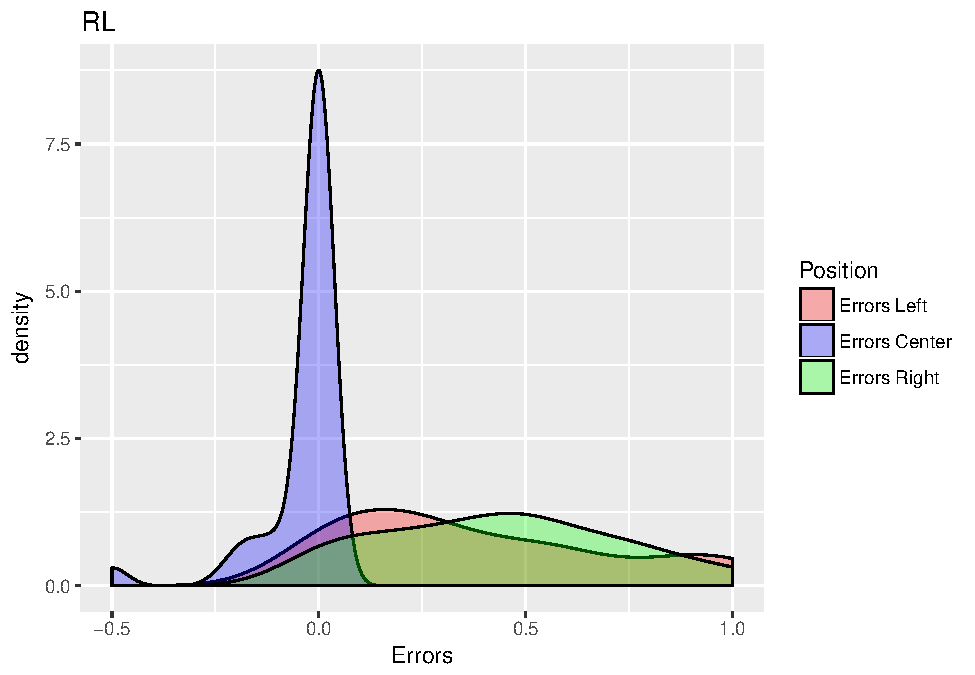
\includegraphics{individual_analysis_report_files/figure-latex/unnamed-chunk-9-5.pdf}

\begin{verbatim}
## Warning: Removed 2 rows containing non-finite values (stat_density).
\end{verbatim}

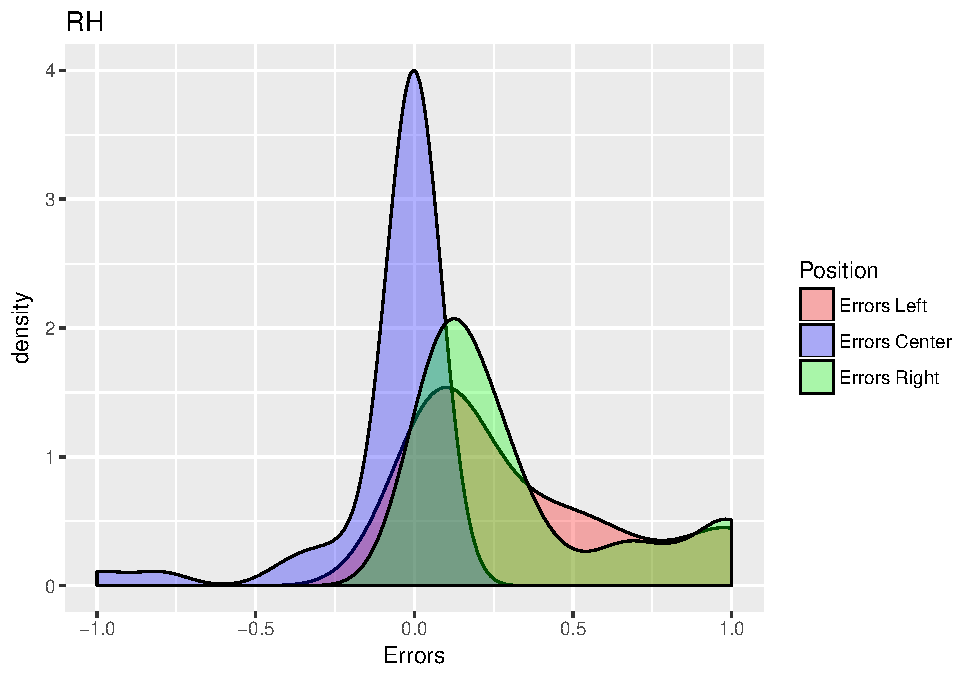
\includegraphics{individual_analysis_report_files/figure-latex/unnamed-chunk-9-6.pdf}

According with the graphs, treatmets PH, RL and RH display a similar
behavior in general: overentry in the extreme positions, and less error
in the central one. Among other treatments, there is more
hetereogeneity. In the PLCS treatment, we observe that in extreme
position participants make less mistakes, and error is uniformly
distributed in central position. In the PLCA treatment, there are less
mistakes in the left position, and overentry in the right position.
Finally, in the PL treatment we observe the opposite; more mistakes in
the left positions, and more optimal behavior when participants were in
the right position.

\section{Conclusion}\label{conclusion}

There are differences in the error distributions along the tretments.
This errors reflect the bahavior observed in comparisson with the Nash
Equilibria. In all the treatment, but in PLCS, central position entering
alone was predicted. As we saw in the first graphs, there are diferences
in the entry rate between extreme positions along the treatments and the
errors baheve accordingly; when an extreme position enter more than the
other, the positive error is greater.


\end{document}
